% !TEX root = ../MemPod.tex

\section{Majority Element Algorithm}
\label{sec:MEA}

\begin{figure*}[t]
  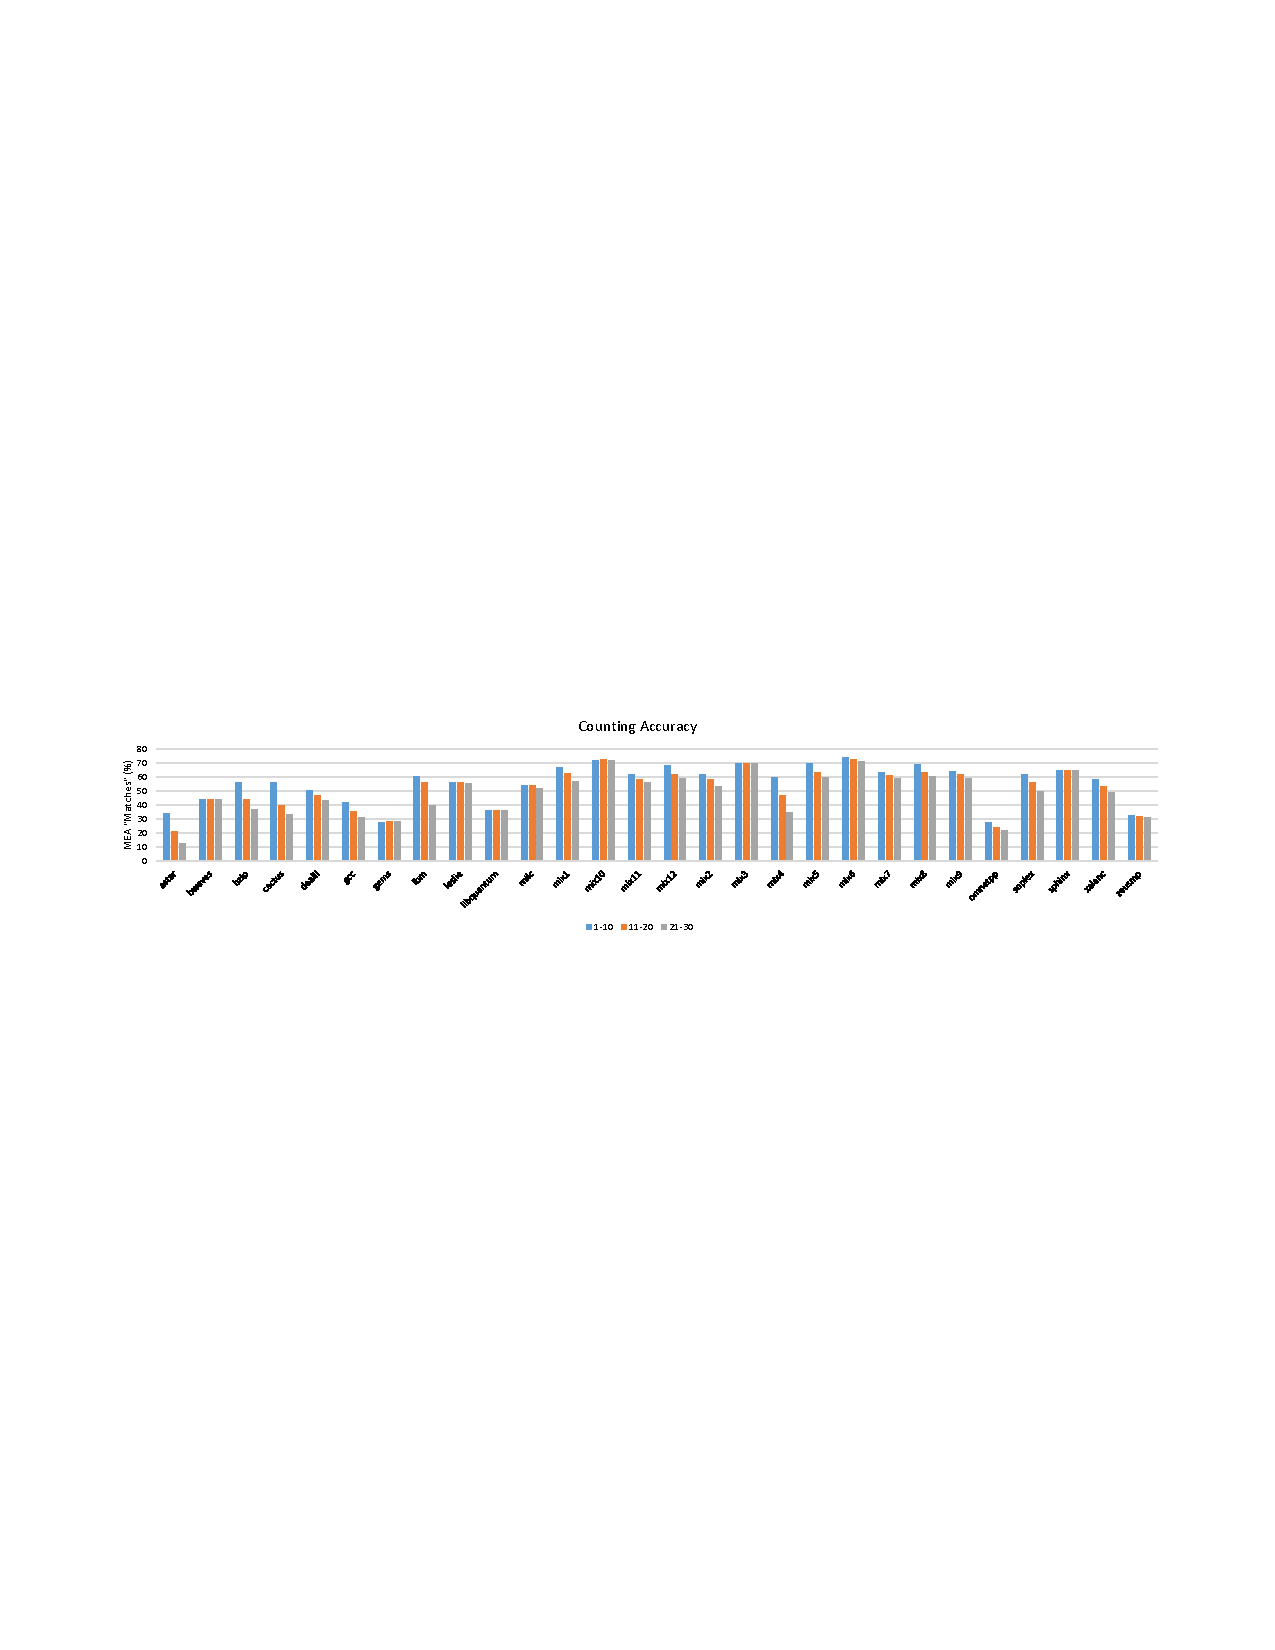
\includegraphics[width=\textwidth]{figures/mea_1.pdf}
  \caption{MEA counting accuracy compared to Full Counters on the top three tiers (ranks 1-10, 11-20, 21-30)}
  \label{fig:mea_1}
\end{figure*}

\begin{figure*}[t]
  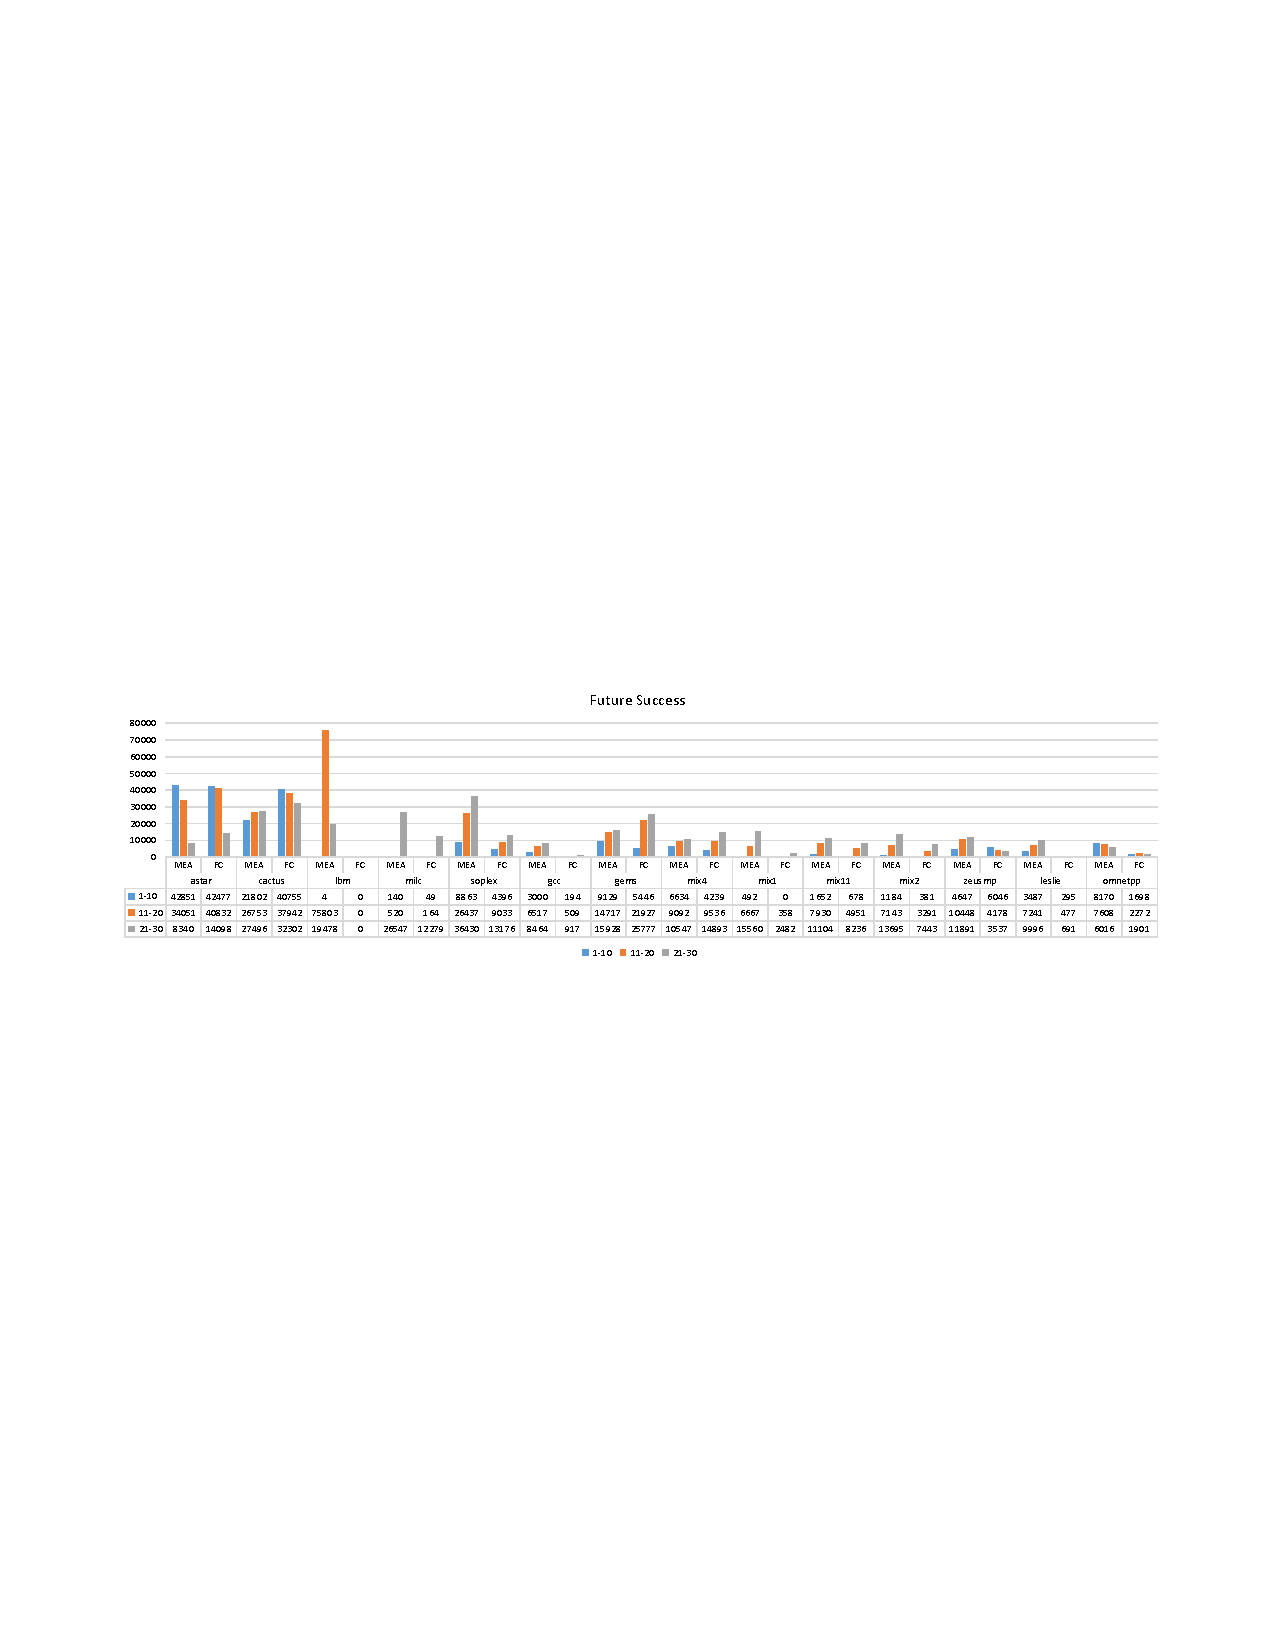
\includegraphics[width=\textwidth]{figures/mea_2.pdf}
  \caption{MEA prediction accuracy (part 1) compared to Full Counters on the top three tiers (ranks 1-10, 11-20, 21-30)}
  \label{fig:mea_2}
\end{figure*}

\begin{figure*}[t]
  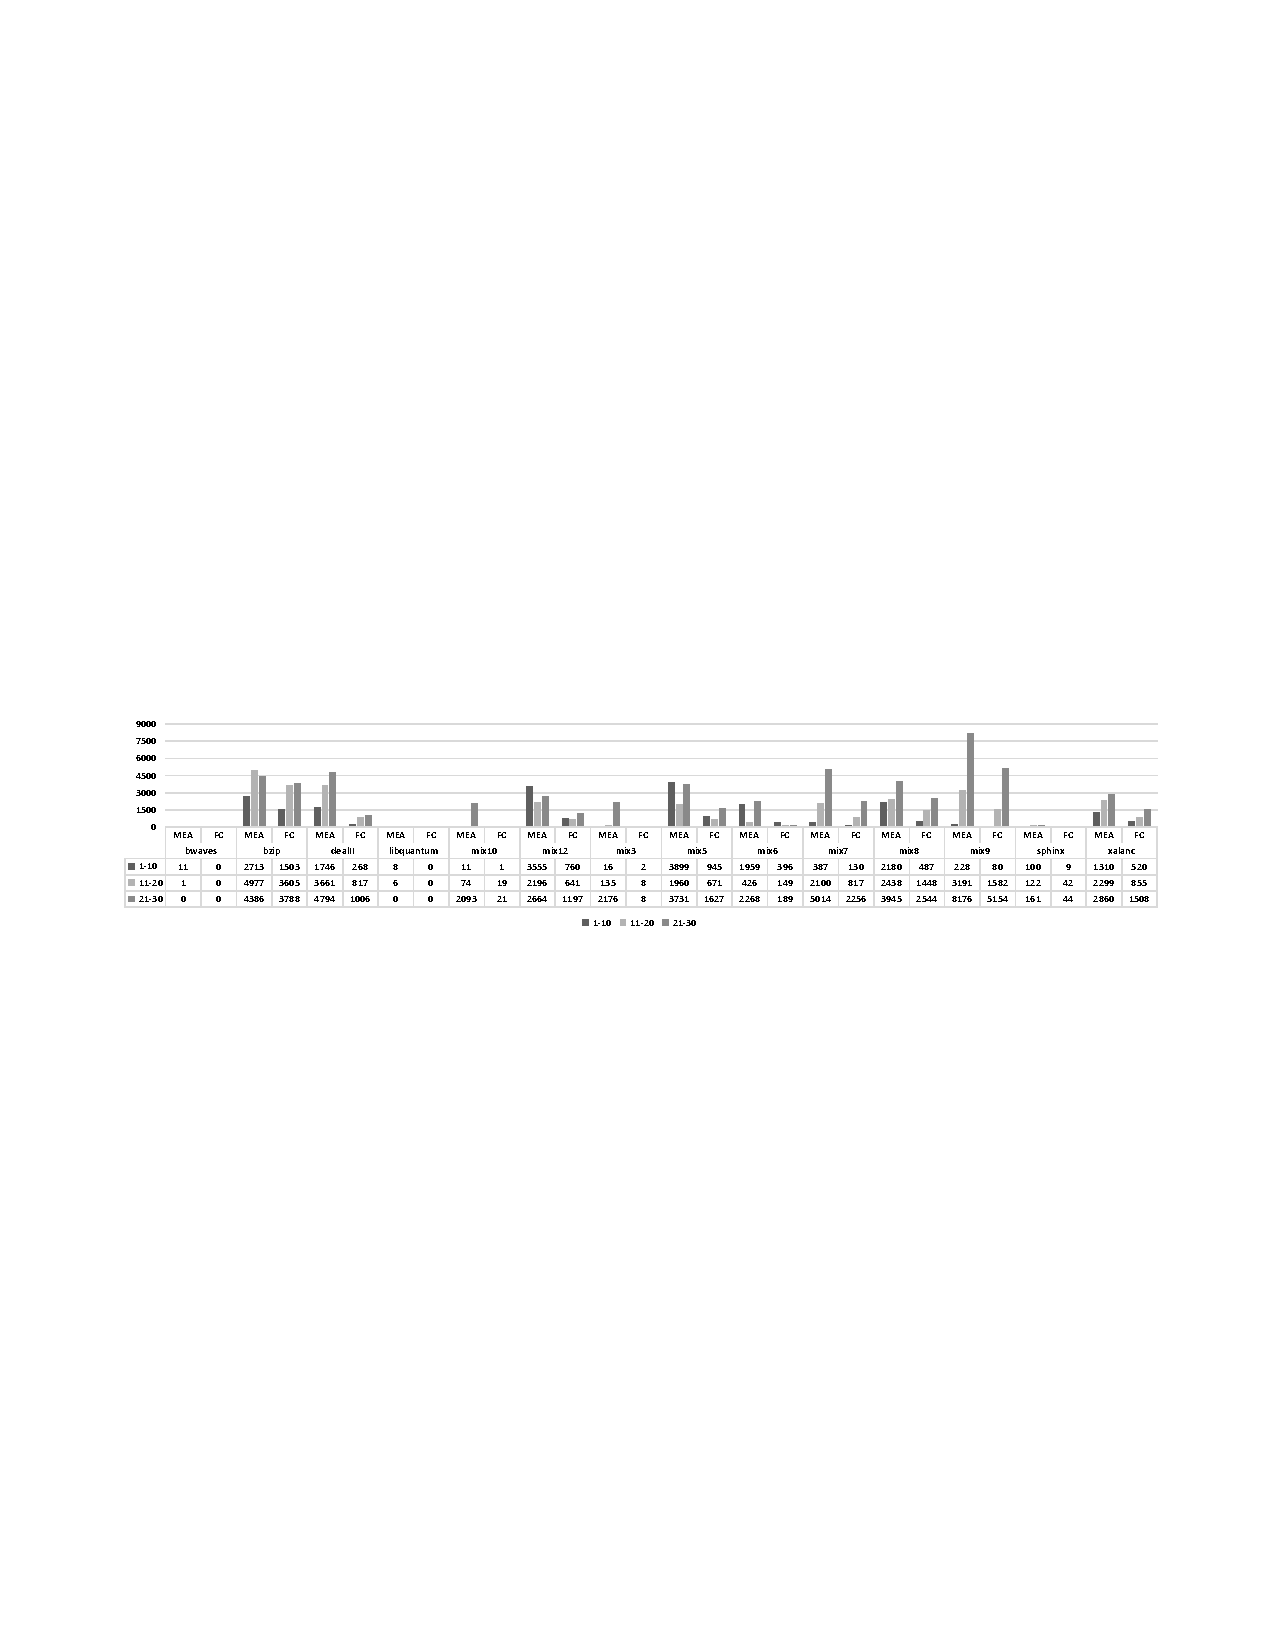
\includegraphics[width=\textwidth]{figures/mea_3.pdf}
  \caption{MEA prediction accuracy (part 2) compared to Full Counters on the top three tiers (ranks 1-10, 11-20, 21-30)}
  \label{fig:mea_3}
\end{figure*}

Memory management mechanisms need the ability to monitor and profile accesses to memory in order to identify hot regions and migrate them. Traditionally, a full set of counters is used, with one counter per physical page -- or region depending on the mechanism's granularity -- in order to accurately keep count of all accesses to all regions. Periodically these counters must be sorted in order to identify the regions with the highest counts. The identified regions will serve as a ``prediction'' for the next interval (i.e. the hottest page of the current interval will be amongst the hottest pages of the following intervals).

MemPod uses the ``Majority Element Algorithm'' $(MEA)$ for its activity tracking needs. MEA attempts to identify the \textit{majority} elements in a set. For example in an array with integers, MEA can be used to identify the \textit{K majority numbers}. Majority elements are the most frequently occurring elements, as long as they exist more than $N \over K+1$ times in the information stream (i.e. they have majority), where N is the number of elements in the array.

The MEA algorithm was originally proposed in \cite{karp-mea} and studied in-depth in \cite{charikar-mea} as a heuristic capable of efficiently identifying majority elements in a stream. This algorithm is formally proven to be 100\% accurate, as long as the K most frequently occurring elements it must identify have majority. With complexity $O(N)$ it could be an ideal candidate for real-time streams of information, such as a stream of memory requests.

\begin{algorithm}
 
 %\DontPrintSemicolon
 \dontprintsemicolon
 \;
 %\PrintSemicolon
 \printsemicolon
 
 \KwIn{X: Set of N elements}
 \KwIn{K: Number of elements to output}
 \KwData{T: Map structure with K entries}
 \KwResult{Set of K majority elements}
 %\DontPrintSemicolon
 \dontprintsemicolon
 \;
 Initialization: $T \leftarrow \emptyset$\; 
 \;
 %\PrintSemicolon
 \printsemicolon
 \ForEach{$i \in X$} {
 	\uIf{$i \in T$}{
		$T[i] \leftarrow T[i] + 1$\;
	}
	\uElseIf{$|T| < K - 1$}{
		$T[i] = 1$\;
	}
	\Else{
		\ForAll{$j \in T$}{
			$T[j] \leftarrow T[j] - 1$\;
			\lIf{$T[j] == 0$}{$T \leftarrow T \setminus {j}$}
		}
	} 
 }
 
 \caption{Majority Element Algorithm}
 \label{alg:mea}
\end{algorithm}

%\begin{algorithm}
%	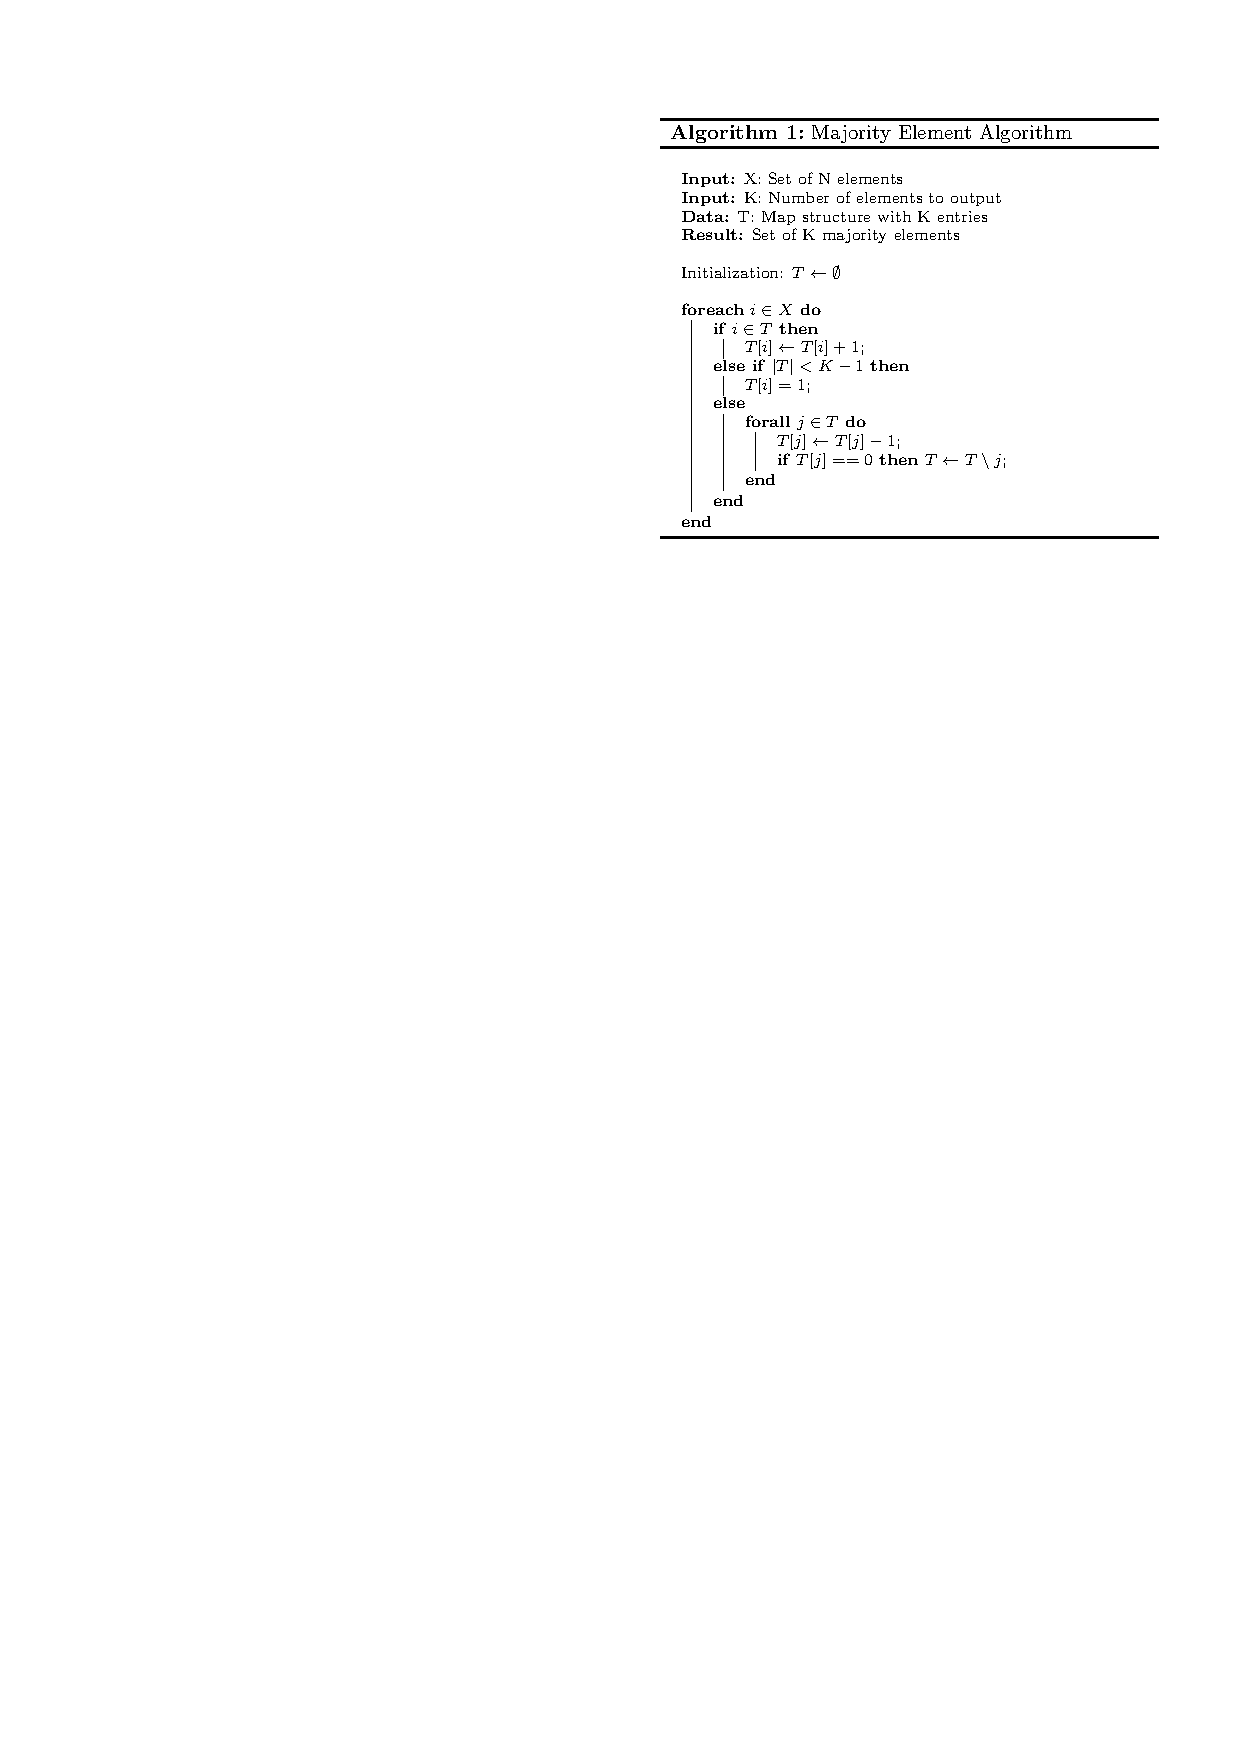
\includegraphics[width=0.45\textwidth]{figures/mea_algorithm.pdf}
%	\caption{TEST}
%	\label{alg:mea}
%\end{algorithm}

The MEA algorithm is presented in Algorithm \ref{alg:mea}: A map structure of K entries holds the element's ID (in our integer array example that would be the integer's value) and maps it to a counter. Looping through the array, if the next integer exists in the map it increases its counter by 1. Otherwise, if there's enough room in the map it adds the new entry with a count of 1. If the number does not exist in the map and all K counters are occupied, the algorithm subtracts 1 from every counter, removes the entries with a counter value of 0 and proceeds to the next integer. Once the entire array is processed, the map entries hold the majority elements.

Even though this heuristic is 100\% accurate, in the absence of its main assumption no guarantees can be made. The outcome of this algorithm relies on several uncontrolled variables, such as the order our requests appeared in. However, the nature of the algorithm presents a very welcomed side effect: Elements accessed repeatedly can be evicted from the map by elements that were accessed less times but more recently. This observation reveals MEA's favoritism towards temporal locality. Furthermore, the area overhead of this algorithm implemented in hardware remains constant, regardless of how many elements need to be profiled (i.e. regardless of how many pages exist in main memory). 

In a memory management scheme that uses Full Counters and a scenario where we want to identify the 100 ``hottest'' pages, we would need one full counter per memory page and on top of that we would have to periodically sort all those counters to pick the top 100. With the use of MEA counters we only need a map with 100 entries regardless of the actual number of pages in main memory. In an 8GB memory with 2kB pages and looking for the top 100 pages, MEA needs $\sim$5K times fewer bits than the full counters' storage requirements (4MB Vs 850B). Considering all the potential benefits MEA can offer in theory, we compared its counting and prediction accuracy against the Full Counters (FC) scheme. 

To evaluate MEA as a possible candidate for activity tracking, we used traces captured from multi-programmed 8-core workloads (the same traces used and described in Section \ref{sec:Results}) and simulated MEA and FC side-by-side with an in-house off-line simulator that provides oracle knowledge of future intervals. The interval size for both MEA and FC was set at 5500 requests which is the average number of requests serviced within a 50us window in our timing experiments. We compared the two mechanisms based on their counting and prediction accuracies regarding the top 3 tiers of memory pages. Pages ranked in the 1-10 hottest pages were grouped in tier 1, tier 2 holds pages ranked 11-20 and finally tier 3 holds pages 21-30.

First we compared MEA's counting accuracy against FC's guaranteed correct counting. In other words we evaluate MEA's capability of identifying the hottest pages of the current interval accurately. Figure \ref{fig:mea_1} shows the counting accuracy of MEA in the top 3 tiers. In the best cases, MEA scored about 75\% accuracy in the top three tiers and about 50\% on average. Our results show that in our use cases MEA is not a viable option in terms of accurate counting. However, correct counting accuracy does not necessarily translate to accurate predictions during future interval(s), even though intuitively, these two aspects might seem correlated.

Figures \ref{fig:mea_2} and \ref{fig:mea_3} present a comparison of MEA and FC in terms of prediction accuracy and demonstrates MEA's true potential. Following the same structure as Figure \ref{fig:mea_1}, we compare each mechanism's ``predictions'' against the top three tiered pages of the following interval (oracle knowledge). First we can observe that in almost all workloads MEA strikes more hits in the top tiered pages. It's also worth noting that FC scored zero in several occasions. In most of those occasions, MEA scored relatively low, but not zero. The \textit{lbm} workload presents a very interesting case. FC was completely unsuccessful in predicting the future, while MEA achieved one of its highest scores throughout all workloads.

Proposed in 2003, to the best of our knowledge, this algorithm has not been used in any micro-architectural proposal before. Our results clearly show that it can well outperform the very expensive option of full counters at greatly reduced hardware cost.
